%%%% For double-blind review submission, w/o CCS and ACM Reference (max submission space)
\documentclass[10pt, sigplan]{acmart}
%%\settopmatter{printfolios=true,printccs=false,printacmref=false}
%% For double-blind review submission, w/ CCS and ACM Reference
%\documentclass[sigplan,10pt,review,anonymous]{acmart}\settopmatter{printfolios=true}
%% For single-blind review submission, w/o CCS and ACM Reference (max submission space)
%\documentclass[sigplan,10pt,review]{acmart}\settopmatter{printfolios=true,printccs=false,printacmref=false}
%% For single-blind review submission, w/ CCS and ACM Reference
%\documentclass[sigplan,10pt,review]{acmart}\settopmatter{printfolios=true}
%% For final camera-ready submission, w/ required CCS and ACM Reference
%\documentclass[sigplan,10pt]{acmart}\settopmatter{}


%% Conference information
%% Supplied to authors by publisher for camera-ready submission;
%% use defaults for review submission.
%\acmConference[PL'17]{ACM SIGPLAN Conference on Programming Languages}{January 01--03, 2017}{New York, NY, USA}
%\acmYear{2017}
%\acmISBN{} % \acmISBN{978-x-xxxx-xxxx-x/YY/MM}
%\acmDOI{} % \acmDOI{10.1145/nnnnnnn.nnnnnnn}
%\startPage{1}

%% Copyright information
%% Supplied to authors (based on authors' rights management selection;
%% see authors.acm.org) by publisher for camera-ready submission;
%% use 'none' for review submission.
\setcopyright{none}
%\setcopyright{acmcopyright}
%\setcopyright{acmlicensed}
%\setcopyright{rightsretained}
%\copyrightyear{2017}           %% If different from \acmYear

%% Bibliography style

%\bibliographystyle{ACM-Reference-Format}

%% Citation style
%\citestyle{acmauthoryear}  %% For author/year citations
\citestyle{acmnumeric}     %% For numeric citations
%\setcitestyle{nosort}      %% With 'acmnumeric', to disable automatic
                            %% sorting of references within a single citation;
                            %% e.g., \cite{Smith99,Carpenter05,Baker12}
                            %% rendered as [14,5,2] rather than [2,5,14].
%\setcitesyle{nocompress}   %% With 'acmnumeric', to disable automatic
                            %% compression of sequential references within a
                            %% single citation;
                            %% e.g., \cite{Baker12,Baker14,Baker16}
                            %% rendered as [2,3,4] rather than [2-4].


%%%%%%%%%%%%%%%%%%%%%%%%%%%%%%%%%%%%%%%%%%%%%%%%%%%%%%%%%%%%%%%%%%%%%%
%% Note: Authors migrating a paper from traditional SIGPLAN
%% proceedings format to PACMPL format must update the
%% '\documentclass' and topmatter commands above; see
%% 'acmart-pacmpl-template.tex'.
%%%%%%%%%%%%%%%%%%%%%%%%%%%%%%%%%%%%%%%%%%%%%%%%%%%%%%%%%%%%%%%%%%%%%%


%% Some recommended packages.
\usepackage{booktabs}   %% For formal tables:
                        %% http://ctan.org/pkg/booktabs
\usepackage{subcaption} %% For complex figures with subfigures/subcaptions
                        %% http://ctan.org/pkg/subcaption
\usepackage{xspace}
\usepackage{graphicx}
\usepackage{ifthen}
\usepackage{pgfplots}
\usepackage{listings}
\usepackage{multirow}
\usepgfplotslibrary{statistics}
\usepackage{dblfloatfix} %enable fig at bottom of page
%\input{macros.tex}

\usepackage{xcolor}
\newcommand{\todo}[1]{\color{orange}\fbox{\bfseries\sffamily\scriptsize TODO:}{\sf\small$\blacktriangleright$\textit{#1}$\blacktriangleleft$}\color{black}}
\newcommand{\sk}[1]{\color{blue}\fbox{\bfseries\sffamily\scriptsize Sophie:}{\sf\small$\blacktriangleright$\textit{#1}$\blacktriangleleft$}\color{black}}
\newcommand{\cba}[1]{\color{purple}\fbox{\bfseries\sffamily\scriptsize Clement:}{\sf\small$\blacktriangleright$\textit{#1}$\blacktriangleleft$}\color{black}}
\newcommand{\eem}[1]{\color{green}\fbox{\bfseries\sffamily\scriptsize Eliot:}{\sf\small$\blacktriangleright$\textit{#1}$\blacktriangleleft$}\color{black}}

%\newcommand*{rotatebox{75}}
\input{macros}

\begin{document}

%% Title information
\title[Garbage Collection Evaluation Infrastructure]{Garbage Collection Evaluation Infrastructure\\ for the Cog VM}

%% Author with single affiliation.
\author{Sophie Kaleba}
                                        %% can be repeated if necessary
\affiliation{
  %\position{Position1}
  \department{Masters student}              %% \department is recommended
  \institution{Universit\'e Lille 1}            %% \institution is required
 % \streetaddress{Street1 Address1}
  \city{Lille}
  %\state{France}
  %\postcode{Post-Code1}
  \country{France}                    %% \country is recommended
}
\email{sophie.kaleba@etudiant.univ-lille1.fr}          %% \email is recommended

%% Author with two affiliations and emails.
\author{Cl\'ement B\'era}
\affiliation{
  % \position{}
	\department{Software Languages Lab}              %% \department is recommended
	\institution{Vrije Universiteit Brussel}            %% \institution is required
	\city{Brussel}
  % \state{}
  % \postcode{}
	\country{Belgium}                    %% \country is recommended
}
\email{clement.bera@vub.ac.be}          %% \email is recommended

%% Author with two affiliations and emails.
\author{Eliot Miranda}
\affiliation{
   \position{Virtual Machine Architect}
	%\department{Virtual Machine architect}              %% \department is recommended
	\institution{Feenk}            %% \institution is required
	\city{San Francisco}
  % \state{}
  % \postcode{}
	\country{California}                    %% \country is recommended
}
\email{eliot.miranda@gmail.com}          %% \email is recommended

\begin{abstract}
One of the next steps to improve Cog, the default virtual machine for multiple programming languages in the Smalltalk family, such as Pharo, Squeak and Newspeak, is to decrease garbage collection pause times. Reference garbage collection algorithm implementations and a benchmarking infrastructure are required to evaluate the performance of a new algorithm and compare it. Cog features a Mark-Compact algorithm, used in production, to which we added a Mark-Sweep algorithm, providing two reference algorithms. Benchmarks are built using two different approaches. Firstly, we turned code from memory intensive deployed applications into benchmarks to simulate real-world applications. Secondly, we built a configurable benchmark which simulates an application with different heap properties to be able to stress specific aspects of the memory management. We then evaluated the two reference algorithms on the infrastructure built to obtain reference benchmark results.
\end{abstract}

\keywords{Benchmark, Garbage Collector, Virtual Machine, Managed Runtime}  %% \keywords are mandatory in final camera-ready submission

\maketitle

\section{Introduction} \label{sec:intro}

The Cog virtual machine (VM), the default VM for multiple programming languages such Pharo \cite{PharoByExample}, Squeak \cite{SqueakByExample} and Newspeak \cite{NewspeakOopsla}, currently features in production a stop-the-world Mark-Compact algorithm as the full garbage collector (GC) algorithm. The algorithm has a high throughput but a high pause time during which the application is not responsive (the GC interrupts the application for multiple seconds on modern Macbooks when using multiple Gbs heaps). For interactive applications, a new algorithm is required with a smaller pause time.

Building and tuning a new GC algorithm requires evaluating its behavior. A benchmarking infrastructure is required to do so. To build GC benchmarks, we took two approaches. 

First, we contacted multiple companies looking for production use of the Cog VM with memory intensive applications ($>$1Gb heaps) and built benchmarks out of one of the deployed applications. As an example, we will discuss in the paper in Section \ref{sec:mooseBench} the Moose benchmarks implemented with the help of Feenk\footnote{https://feenk.com/}. Part of the business of Feenk consists in analysing software written in multiple programming languages using the open-source framework Moose~\cite{MoosePaper1,MooseBook1}. Using Moose, the application parses the software to analyse into a model, performs analysis on it and lastly releases the model. Models currently used are encoded in up to 11Gb. This behaviour was turned into three benchmarks, growing, accessing and shrinking the heap. 

Second, we implemented a configurable benchmark: the idea is to set-up specific heap characteristics that will stress the garbage collector. A set of options is available to the user to tune the type of allocated objects and some of their features. These options can be associated with different heap states: growing, stable or shrinking, like in our other approach. We ran two benchmark cases with this tool: large objects in heap and majority of data objects in heap.
This implementation and the use-cases are detailed in Section \ref{sec:confBench}

To evaluate a new algorithm, we also need to compare it to reference implementations. The Cog VM features a Mark-Compact algorithm used in production. The compaction phase is quite specific since it slides objects down in memory while handling pinned objects and spends time updating references to point to their eventual locations. In addition to this algorithm, we implemented a Mark-Sweep, which does not move objects in memory and is thus quicker to perform. Section \ref{sec:ref} details the two implementations.

We evaluated both algorithms on the benchmarks we built to provide results of the reference algorithms on the infrastructure built.

We conclude the paper by discussing some related work, the GC benchmarks suites for Java and the ACDC benchmarks, and some future work.

\section{Building Benchmarks} \label{sec:bench}
Experience with applications deployed on Cog shows that memory intensive applications often exhibit three distinct regimes.  As an application builds a new data structure the heap grows, and the garbage collector should be biassed to allow growth, rather than to favour performing garbage collection when the current size of the heap is reached.  As an application processes the data structure it has built the heap is stable, at least in its size.  If the application then releases significant storage and continues processing, the garbage collector should favour reclamation, and it is advantageous if it attempts to free up memory segments and return them to the OS.  We have identified, therefore, growing, stable and shrinking regimes, and these are useful abstractions of real application behaviour, which are helpful in designing meaningful benchmarks and in providing tuning mechanisms to the system programmer.

To build GC benchmarks, we took two approaches. We asked companies for their deployed memory intensive applications and turned them into benchmarks. Multiple benchmarks in this category include closed-source code. In Section \ref{sec:mooseBench}, we describe how we turned a specific application into a benchmark with the help of the company (this specific benchmark does not include closed-source code). Then, to stress the GC on specific aspects, we built a configurable benchmark that based on the configuration emulates heaps with different properties. 

\subsection{Moose benchmark} \label{sec:mooseBench}

Part of the business of Feenk consists in analyzing large software systems. To do so, the application parses a mse file into a model (mse is the default file format supported by Moose), performs some analysis, and then releases the model and generates analysis results. For business, the application analyzes closed-sourced application of companies. To build an open-source benchmark, we analyse open-source applications instead of closed-source ones.

We built four different benchmarks that fall into three categories: growing, stable and shrinking heaps. The benchmarks were built on top of the stable Moose image\footnote{http://www.moosetechnology.org/}.

\paragraph{Growing heap.} The growing heap benchmarks increase the heap size as they are performed, mainly creating objects. We built two benchmarks:
\begin{itemize}
	\item \emph{LoadFromMSE}: parses a mse file into a moose model, effectively loading a graph of objects. This is the only benchmark not taking a moose model as a parameter.
	\item \emph{ExpandProperties}: computes all interesting properties of the model, discarding properties rarely used or consuming too much memory, cacheing common properties not using too much memory. It effectively loads a graph of objects connected in many points to the original graph. 
\end{itemize}

\paragraph{Stable heap.} The stable heap benchmarks perform random memory accesses in a heap whose size remains approximately the same. We built one benchmark, \emph{ExpandPropertiesWithCache}, which computes all interesting properties of the model, common properties with low memory footprint are already cached and other properties are discarded once computed.

\paragraph{Shrinking heap.} The shrinking heap benchmark frees part of the heap and performs a GC. We built only one benchmark, \emph{Release}, which removes references to the graph of objects and performs three garbage collections.

\subsection{Configurable Benchmark} \label{sec:confBench}

Running a new memory management strategy on real-world applications can give an early insight into its performance. Being able to configure a specific set-up allows stressing specific behaviors of the new implementation.
This configurable benchmarking tool has been implemented to emulate specific heap characteristics and states potentially to trigger edge cases. The user has available a set of twelve options which can be sorted into two categories:

\paragraph{Heap characteristics.} A first set of options allows the user to modify the heap characteristics, i.e.\ the amount and sizes of objects to allocate and the possible interactions with these objects. 

\begin{itemize}
\item \emph{wantedAllocatedSize:} the cumulative size (in Kb) of objects that will be allocated.
\item \emph{minSize and maxSize:} the minimum and maximum sizes of objects.
\item \emph{dataObjects, weakStructures, classes, compiledMethods, ephemerons:} the ratio for each of these object types.
\item \emph{accessObjects:} if set to True, access half of the objects allocated on the heap .
\item \emph{readOnly:} if set to False, modify half of the objects allocated on the heap upon accessing.
\end{itemize}

\paragraph{Heap state.} The heap state can also be tuned. Once objects have been allocated on the heap according to the selected options, it is possible to decide whether to allocate more objects (growing heap), to release objects that have been previously allocated (shrinking heap), or to stay in the current state and potentially access and modify objects that have been previously allocated (stable heap). These options echo the 3 benchmarks depicted in Section \ref{sec:mooseBench}\\

We built two benchmarks out of the potential configurations:
\begin{itemize}
\item \emph{LargeObjects:} Only large objects with a size greater than 65535 32-bit machine words are allocated on the heap. These objects are allocated directly in the old space.
\item \emph{Data0bjects:} The majority of the objects that will be allocated on the heap will be Data objects, which will only contain one-byte-sized integers in this benchmark. Data Objects are raw data objects, which can be used, for example, to store characters, restricted-range integers, floats, etc: the garbage collector will not go through their slots in the marking phase.
\end{itemize}

\section{Reference Implementations} \label{sec:ref}

To evaluate new full GC algorithms, we need to compare it against existing algorithms. Two of the most common GC algorithms are Mark-Compact and Mark-Sweep. We describe here the current Mark-Compact implementation, which has been in production for the past few years, and an implementation of Mark-Sweep we introduced as a reference earlier this year.

Cog is written to allow new object representations to be written and used.  Spur \cite{SpurMirandaBera} is the second object representation written for Cog.  Spur avoids the cost of an explicit read barrier to follow forwarding pointers on most accesses by handling the forwarding check on the failure side of cached dynamic message send; any send to a forwarded object will fail, and forwarding pointers in the current frame are followed on the failure side of lookup.  Hence in Spur all objects have room for a forwarding pointer.  This is key to the implementation of the Mark-Compact algorithm. 

\subsection{Mark-Compact} \label{sec:refmc}


Cog's Mark-Compact algorithm, named \emph{SpurPlanningCompactor}, implements the classic planning compaction algorithm for Spur.  It uses the fact that there is room for a forwarding pointer in all objects to store the eventual position of an object in the first field. It therefore first locates a large free chunk, or the Eden space or a memory segment, to use as the savedFirstFieldsSpace, which it uses to store the first fields of objects that will be compacted, these fields being overwritten by each object's eventual position. It then makes at least three passes through the heap.

The first pass plans where live movable objects will go, copying the first field to the next slot in savedFirstFieldsSpace, and setting the forwarding pointer to point to the object's eventual location. The second pass updates all pointers in live pointer objects to point to objects' final destinations, including the fields in savedFirstFieldsSpace. The third pass moves objects to their final positions, unmarking objects, and restoring saved first fields as it does so. If the forwarding fields of live objects in the to-be-moved portion of the entire heap won't fit in savedFirstFieldsSpace, then additional passes can be made until the entire heap has been compacted.  When snapshotting (saving the system to a file for later resumption, see below) multiple passes are made, but when doing a normal GC only a single pass is made.

Each pass uses a three finger algorithm, a simple extension of the classic two finger algorithm \cite{Cheney} with an extra middle finger used to refer to the lowest pinned object, if any, between the to and from fingers.  Objects are moved down, starting at the first free object or chunk, provided that they fit below the lowest pinned object above the to finger.  When an object won't fit the to finger is moved above the pinned object and the third finger is reset to the next pinned object below the from finger, if any.  The scheme preserves object order amongst movable objects, making no attempt to fit objects in any gaps left below pinned objects.

\subsection{Mark-Sweep} \label{sec:refms}

Cog's Mark-Sweep algorithm, named \emph{SpurSweeper}, is a sweep-only algorithm.  Setting the compactor to SpurSweeper effectively changes the fullGC to a mark-sweep non-moving algorithm. It iterates over all objects in old space in linear order. Each time an unmarked object or a free chunk is met, it coalesces it with subsequent ones and updates the free lists with a new larger free chunk.

\subsection{Mark-SelectiveCompact}
We added a new algorithm designed to reduce the pause time due to compaction.  This algorithm, to be described fully elsewhere, chooses sparsely populated segments and compacts these to an empty segment to reduce fragmentation.  It relies on Spur's implicit following of forwarding pointers to update references to moved objects without requiring a complete pass over the heap. 

\subsection{Snapshot discussion}

On top of the Cog VM, snapshots can be performed to persist the given state of the heap. Since snapshots are persisted, they should use a low amount of memory to avoid using too many bytes on disk. Non compacting algorithms, such as the Mark-Sweep, or algorithms compacting only part of the heap, such as garbage first~\cite{G1}, are a problem in this context. The heap, when collected by the Mark-Sweep, has a lot of free chunks when the heap size varies a lot leading to a large snapshot. However, the non compacting algorithm also has interesting advantages, for  example lower garbage collection pause times. 

To be able to have a garbage collector with a low pause time and still be able to perform snapshots efficiently, we designed a hybrid compactor solution which includes both SpurSelectiveCompactor and SpurPlanningCompactor. The VM tells the hybrid compactor if the garbage collection is to be performed for snapshot or not, and the compactor chooses to apply one algorithm or the other to achieve either a low compaction pause time or a snapshot with a minimised memory footprint.

\section{Reference Results} \label{sec:valid}

We evaluated both reference algorithms on the benchmarks built. 

In the results, the compaction time includes the time spent in the compact phase in the Mark-Compact and in the sweep phase in the Mark-Sweep. Total full GC time is the total time spent in full GCs, including  compaction time. Scavenge time is the time spent in scavenging, \emph{i.e.,} garbage collection of young objects only. Total execution time is the total execution time, including scavenge and full GC time. Scavenge time is drastically smaller with a larger Eden, leading to better overall performance.

\subsection{Moose Benchmarks}


\paragraph{Set-up.}The Moose benchmark evaluation was performed on a MacBook pro running Mac OS 10.11.6, with a 2.9 Ghz Intel Core i5 processor, and 8 Gb of  1867MHz DDR3 RAM. The Mac VM was compiled using Apple LLVM version 8.0.0 (clang-800.0.38). The compiled VMs are native 64 bit applications with 64-bit objects and pointers.

We evaluated the Moose benchmarks using the reference Mark-Compact and Mark-Sweep algorithms and by analysing the wildfly code base\footnote{http://www.wildfly.org/}. We distinguish four configurations:
\begin{itemize}
\item \emph{Sweep}: VM with standard GC parameters and the Mark-Sweep algorithm.
\item \emph{Compact}: VM with standard GC parameters and the Mark-Compact algorithm.
\item \emph{Compact-16}: VM with standard GC parameters, except Eden size which is 16 times larger, and the Mark-Compact algorithm.
\item \emph{Sweep-16}: VM with standard GC parameters, except Eden size which is 16 times larger, and the Mark-Sweep algorithm.
\end{itemize}
With a larger Eden, more overall memory is used (in our case an extra 90 Mb), but scavenge time is expected to be lower. The Spur scavenger is an extended implementation of Ungar's classic generation scavenger~\cite{Scavenger} and the scavenge time is proportional to the number of surviving objects.
%To evaluate the performance, we use:
%\begin{itemize}
%	\item the production VM generated by the CI of opensmalltalk-vm\footnote{https://github.com/OpenSmalltalk/opensmalltalk-vm}, that we call Mark-Compact or Compact.
%	\item a custom compiled VM, which features a different compactor, that we call Mark-Sweep or Sweep.
%\end{itemize}

%
\begin{figure*}[thb]
	\centering
    
    \begin{subfigure}[b]{.48\textwidth}
	\includegraphics[width=\linewidth]{figures/load} 
	\caption{LoadFromMSE\vspace{0.2cm}}
   	\end{subfigure}\hspace{0.03\textwidth}% 
   	\begin{subfigure}[b]{.48\textwidth}
	\includegraphics[width=\linewidth]{figures/prop} 
	\caption{ExpandProperties\vspace{0.2cm}}
   	\end{subfigure}	
	\begin{subfigure}[b]{.48\textwidth}
	\includegraphics[width=\linewidth]{figures/propCache} 
	\caption{ExpandPropertiesWithCache}
	\end{subfigure}\hspace{0.03\textwidth}%
	   	\begin{subfigure}[b]{.48\textwidth}
	\includegraphics[width=\linewidth]{figures/release} 
	\caption{Release}
   	\end{subfigure}

   	   	    	
\caption{Moose benchmark results piled up (in ms).} \label{MooseRes1}
\end{figure*}

\begin{figure*}[thb]
\begin{tabular}{|c|c|l|l|l|l|l|l|}
   \hline
  & & Total   & Scavenge  & Total Full  & Compaction  & Initial  & Final \\
 Benchmark & &  Exec. time &  time & GC time &  time &  Heap size & Heap size \\
  & &  (ms) &  (ms) & (ms) &  (ms) &  (Mb) &  (Mb) \\
   \hline
   \multirow{4}{*}{LoadFromMSE} & Sweep 	& 159821 $\pm$ 2218 &	73599 $\pm$ 1281 	& 10863 $\pm$ 726 	&1398 $\pm$ 91 	& 193 $\pm$ 0 	& 959 $\pm$ 9.69 \\
    				    & Compact 	& 162305 $\pm$ 2790 &	72150 $\pm$ 782 	& 14091 $\pm$ 972 	&4661 $\pm$ 289 	& 193 $\pm$ 0 	& 909 $\pm$ 9.69 \\
    				    & Compact-16 	& 96043 $\pm$ 540 &	14279 $\pm$ 124 	& 12440 $\pm$ 217 	&5575 $\pm$ 36 	& 283 $\pm$ 0 	& 1055 $\pm$ 0 \\
    				    & Sweep-16 		& 91721 $\pm$ 1131 &	13862 $\pm$ 49 	& 9352 $\pm$ 73 	&1208 $\pm$ 9 	& 283 $\pm$ 0 	& 988 $\pm$ 0 \\
   \hline
   \multirow{4}{*}{ExpandProperties} 	& Sweep 		& 232940 $\pm$ 1287 &	55497 $\pm$ 238 	& 12240 $\pm$ 285 	&1178 $\pm$ 6.66 	& 959 $\pm$ 9.69 & 1888 $\pm$ 0 \\
    				    			& Compact 	& 183314 $\pm$ 13090 &	53165 $\pm$ 2343 	& 12496 $\pm$ 197 	&3775 $\pm$ 108 	& 909 $\pm$ 9.69 & 1938 $\pm$ 0 \\
    				    & Compact-16 	& 100315 $\pm$ 138 &	9372 $\pm$ 75 	& 9466 $\pm$ 87 	&3301 $\pm$ 31 	& 1055 $\pm$ 0 	& 2028 $\pm$ 0 \\
    				    & Sweep-16 		& 107914 $\pm$ 216 &	9714 $\pm$ 34 	& 9384 $\pm$ 107 	&864 $\pm$ 5 	& 988 $\pm$ 0 	& 2011 $\pm$ 0 \\
   \hline
    					& Sweep 		& 510013 $\pm$ 5812 	&	64234 $\pm$ 823 	& 23225 $\pm$ 100 	&2011 $\pm$ 10 	& 1888 $\pm$ 0 	& 1888 $\pm$ 0 \\
     	ExpandProperties	& Compact 	& 408169 $\pm$ 20444 	&	64492 $\pm$ 1234 	& 0 $\pm$ 0 		&0 $\pm$ 0 		& 1938 $\pm$ 0 	& 1938 $\pm$ 0 \\
    		WithCache	& Compact-16 	& 105389 $\pm$ 1067 	&	6467 $\pm$ 47 		& 3019 $\pm$ 24 	&937 $\pm$ 6 		& 2028 $\pm$ 0 	& 2028 $\pm$ 0 \\
    				    	& Sweep-16 	& 114325 $\pm$ 403 	&	6323 $\pm$ 23 		& 2347 $\pm$ 13 	&209 $\pm$ 6 		& 2011 $\pm$ 0 	& 2011 $\pm$ 0 \\
   \hline
   \multirow{4}{*}{Release} 	& Sweep 		& 606 $\pm$ 16 		&	0 $\pm$ 0 	& 605 $\pm$ 16 	&316 $\pm$ 12 		& 1888 $\pm$ 0 		& 534 $\pm$ 58 \\
    				    		& Compact 	& 1092 $\pm$ 2 		&	0 $\pm$ 0 	& 1092 $\pm$ 1 	&806 $\pm$ 3 			& 1938 $\pm$ 0 		& 193 $\pm$ 0 \\
    				    & Compact-16 	& 1120 $\pm$ 13 		&	0 $\pm$ 0 		& 1119 $\pm$ 13 	&829 $\pm$ 8 			& 2028 $\pm$ 0 		& 300 $\pm$ 0 \\
    				    & Sweep-16 		& 610 $\pm$ 1 			&	0 $\pm$ 0 		& 610 $\pm$ 1 		&314 $\pm$ 2 			& 2011 $\pm$ 0 		& 535 $\pm$ 203 \\
   \hline
\end{tabular} 
\caption{Moose benchmark results with standard errors.} \label{MooseRes2}
\end{figure*}

The results are shown in Figure \ref{MooseRes1} and \ref{MooseRes2}. 

\paragraph{LoadFromMSE.} The LoadFromMSE benchmark grows the memory by around 700Mb. Compaction time is smaller for the sweep algorithm, making the benchmark a little bit faster in the Mark-Sweep, which is to be expected since Sweep does not need to waste time updating pointers because objects are not moved in memory.

\paragraph{ExpandProperties.} The ExpandProperties benchmark grows the memory by around 1 Gb. Compaction time is a little bit better with the sweep algorithm as for the previous benchmark, but execution time is much worse. We believe this is due to worse locality of objects. With a larger Eden,  scavenge time is much smaller and the execution time is a bit faster due to improved object locality.

\paragraph{ExpandPropertiesWithCache.} The ExpandProperties WithCache benchmark does not increase the overall memory size. Since the compacting GC has compacted the heap before starting the benchmark, there is enough room to allocate the large objects required by the benchmark (large objects are allocated directly in old space) and there is no need for a full GC during the benchmark. However, with the sweep algorithm, there are multiple small free memory chunks which are not big enough to hold all the requested large objects, so a full GC is required. In addition, execution time is worse, as for the previous benchmark. With a larger Eden, the scavenge time is much smaller and the execution time is much faster due to improved object locality.

\paragraph{Release.} The Release benchmark releases all the graphs. With the compacting GC, memory goes back to its original size. With Sweep, multiple memory segments are left with a few live objects, preventing the VM from returning those segments to the OS. Hence, the memory decreases drastically, but not to the original size. Compaction time is much faster with Sweep, but as we have discussed, for less efficiency. Changing Eden size has little if any impact here, since it's essentially a pure full GC benchmark.


\begin{figure*}[b!]
	\centering
    
    \begin{subfigure}[b]{.499\textwidth}
	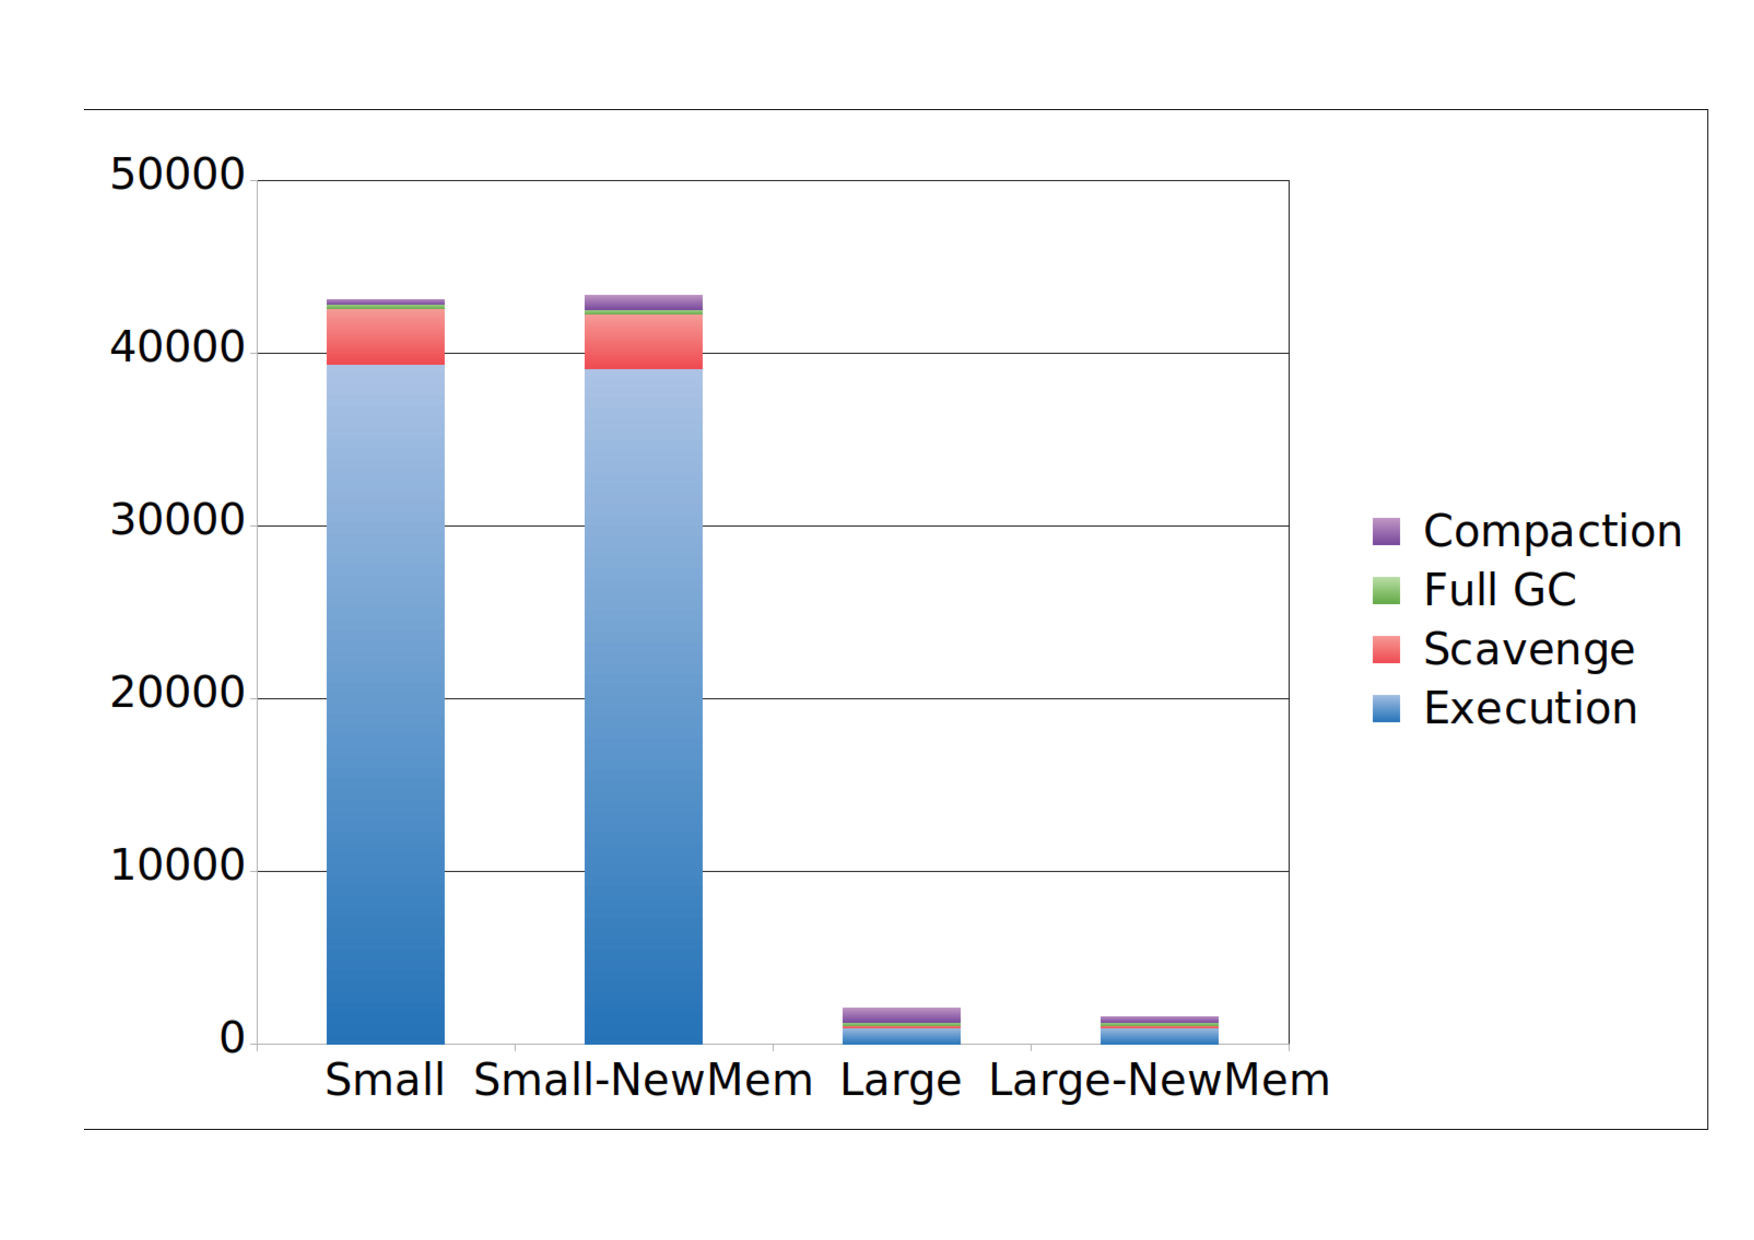
\includegraphics[width=\linewidth]{figures/large} 
	\caption{LargeObjects\vspace{0.2cm}}
   	\end{subfigure}\hspace{0.00000001\textwidth}% 
   	\begin{subfigure}[b]{.499\textwidth}
	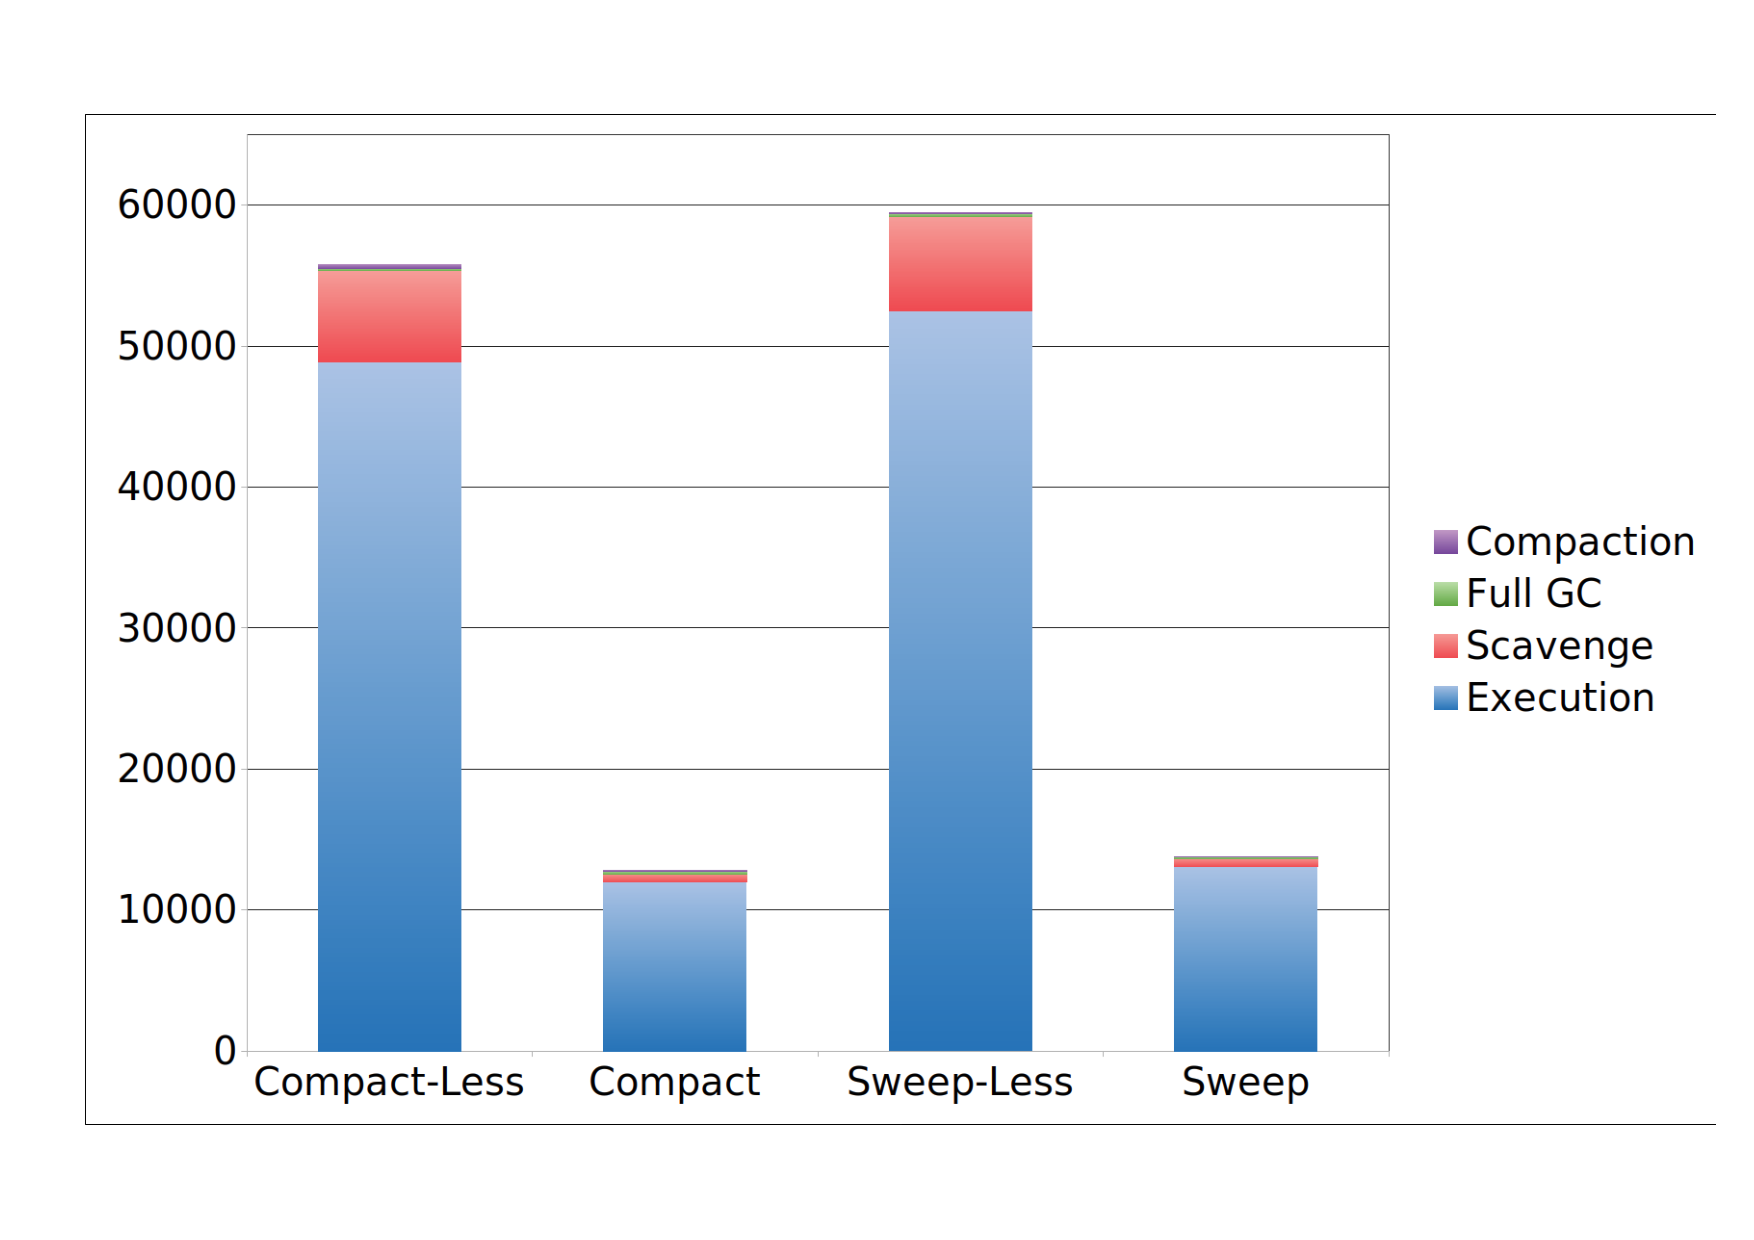
\includegraphics[width=\linewidth]{figures/data} 
	\caption{DataObjects\vspace{0.2cm}}
   	\end{subfigure}	

   	   	    	
\caption{Configurable benchmark results piled up (in ms).} \label{ConfigRes1}
\end{figure*}

\begin{figure*}[b!]
\begin{tabular}{|c|c|l|l|l|l|}
   \hline
  & & Total   & Scavenge  & Total Full  & Compaction   \\
 Benchmark & &  Exec. time &  time & GC time &  time \\
  & &  (ms) &  (ms) & (ms) &  (ms)\\
   \hline
   \multirow{4}{*}{LargeObjects} & Small 	& 43110 $\pm$ 338 &	3223 $\pm$ 76 	& 541 $\pm$ 5 	&298 $\pm$ 2.8  \\
    				    & Small-NewMem 	& 42886 $\pm$ 341 &	3204 $\pm$ 23 	& 605 $\pm$ 43 	&348 $\pm$ 8  \\
    				    & Large 	& 1514 $\pm$ 15 &	155 $\pm$ 4 	& 414 $\pm$ 1 	&223 $\pm$ 4  \\
    				    & Large-NewMem 		& 1506 $\pm$ 20 &	163 $\pm$ 8 	& 408 $\pm$ 6 	&219 $\pm$ 6  \\
   \hline
   \multirow{4}{*}{DataObjects} 	& Compact-Less 		& 55757 $\pm$ 1998 &	6465 $\pm$ 122 	& 403 $\pm$ 36 	&232 $\pm$ 20.55  \\
    				    			& Compact 	& 12738 $\pm$ 13090 &	569 $\pm$ 10 	& 168 $\pm$ 27 	&98 $\pm$ 15  \\
    				    & Sweep 	& 13785 $\pm$ 269 &	604 $\pm$ 9 	& 115 $\pm$ 2 	&27 $\pm$ 1 \\
    				    & Sweep-Less 		& 59398 $\pm$ 592 &	6679 $\pm$ 34 	& 226 $\pm$ 3 	&56 $\pm$ 1 \\

   \hline
\end{tabular} 
\caption{Configurable benchmark results with standard errors.} \label{ConfigRes2}
\end{figure*}


\subsection{Configurable Benchmark}

\paragraph{Set-up.}The Configurable Benchmark evaluation was performed on an Asus Zenbook running Ubuntu 18.04 LTS, with a 2.2 Ghz processor Intel Core i5, and 8 Gb of 1600MHz DDR3 RAM. The Linux VM was compiled using GCC version 5.4.0. The compiled VMs are 32-bit (x86) applications with 32-bit objects and pointers. \footnote{Spur uses a common object header for both 32-bit and 64-bit versions, so 32-bit objects still have a 64-bit header and are all aligned on a 64-bit boundary.}


We evaluated the configurable benchmarks using the reference Mark-Compact and Mark-Sweep algorithms and by generating specific heap configurations. 
The results are shown in Figure \ref{ConfigRes1} and \ref{ConfigRes2}.

\paragraph{LargeObjects.} The LargeObjects benchmark compares the time spent in garbage collection according to the size of allocated objects. We distinguish four configurations:
\begin{itemize}
\item \emph{Small}: VM with standard GC parameters and the Mark-Compact algorithm. Objects smaller than 65535 32-bit machine words are allocated.
\item \emph{Small-NewMem}: VM with standard GC parameters, except segment size which is 4 times larger, number of empty segments which is multiplied by 4, and the Mark-Compact algorithm. Objects smaller than 65535 32-bit machine words are allocated.
\item \emph{Large}: VM with standard GC parameters and the Mark-Compact algorithm. Objects larger than 65535 32-bit machine words are allocated.
\item \emph{Large-NewMem}: VM with standard GC parameters, except segment size which is 4 times larger, number of empty segments which is multiplied by 4, and the Mark-Compact algorithm. Objects larger than 65535 32-bit machine words are allocated.
\end{itemize}
The time spent in scavenging is lower for the larger objects. Allocating large objects has an impact on the number of memory growing and shrinking operations, which can be altered by tuning the associated parameters in the VM. 
\paragraph{Data0bjects.} The DataObjects benchmark compares the time spent in garbage collection according to the amount of allocated data objects.
We distinguish four configurations:
\begin{itemize}
\item \emph{Compact-Less}: VM with standard GC parameters and the Mark-Compact algorithm. 40\% of allocated objects are data objects.
\item \emph{Compact}: VM with standard GC parameters and the Mark-Compact algorithm. 90\% of allocated objects are data objects.
\item \emph{Sweep-Less}: VM with standard GC parameters and the Mark-Sweep algorithm. 40\% of allocated objects are data objects.
\item \emph{Sweep}: VM with standard GC parameters and the Mark-Sweep algorithm. 
90\% of allocated objects are data objects.
\end{itemize}
 The time spent in full GC's and the compaction time are lower in comparison with a case with 40\% of Data Objects. This can be explained because less time is spent in the marking and pointer update phases.

\section{Related and Future Work}

\paragraph{GC benchmark suite.} The DaCapo benchmark suite \cite{DacapoBench} is a standard set of benchmarks designed for Java applications. It gathers together several open-source benchmarks and runs them against specific metrics to assess their potential significance towards different aspects of the Java language implementation, typically its memory management and virtual machines.
With regard to memory management, the eleven benchmarks selected in 2006 (and updated later in 2009 to add three more benchmarks \cite{DaCapo}) are assessed according to the number of allocated objects, their average size, and the maximum number of live objects. The nursery (new space) survival rate is also taken into account, as well as the heap structure through object lifetime behavior.

\paragraph{ACDC-JS.}
ACDC-JS \cite{ACDCJS} is a configurable \\benchmarking tool designed to measure and stress allocation and deallocation time in the JavaScript memory management model. 
It builds a heap model based on the behavior of real-world applications and aims at providing significant insights into JavaScript memory management that cannot be obtained from standard benchmarking suites. The value of specific heap options can be set by the user. 
Their study shows the negative impact of object liveness (time between allocation and last access, leading to the objects to be in different spaces in the heap) and deallocation delay on allocation time. It also stresses the trade-offs between memory consumption and allocation latency.

\paragraph{Future work: more benchmarks.}
We described two approaches to bench new memory management strategies: the Moose benchmark, based on a real-world application and the configurable benchmarking tool, highlighting edge cases by stressing the garbage collector on specific aspects. It would be nice to add some benchmarks based on the standard DaCapo benchmark suite so we could assess the performance of our memory management strategies via a reputed benchmarking suite.

\paragraph{Future work: stress GC tests.}
We can stress the garbage collector by running the configurable benchmarking tool with specific sets of options to test the memory startegy in edge cases. By increasing the amount of edge-cases benchmarks led on the garbage collector, we could infer a serie of tests to secure the garbage collector behaviour in these situations.

\paragraph{Future work: more options.}
The number of options available in the configurable tool is still limited at the moment. We can take advantage of the ACDC-JS implementation, as well as some metrics used in the DaCapo paper, to get a higher number of options and improve the data collected during the benchmark.

\paragraph{Future work: incremental GC.}
This investigation, including as it does a framework for compaction that includes a new store check, helps us in designing a fully incremental Mark-Sweep-Compact algorithm for Spur with very low pause times, suitable for interactive applications such as animation and gaming.


\section*{Acknowledgments}
We thank Tudor Girba for providing the files needed for the Moose benchmark.


%% Bibliography
\bibliographystyle{alpha}
\bibliography{sista}


\end{document}
